% どうやって解くかの説明

\section{研究の目的}
\begin{frame}
  \frametitle{研究の目的}

  \begin{block}{\textbf{表現力}と\textbf{安全性}を兼ね備えたコード生成言語の構築}
    \begin{itemize}
    \item 表現力: 多段階let挿入,メモ化等の技法を表現
    \item 安全性: 生成されるコードの一定の性質を静的に検査
    \end{itemize}
  \end{block}

  \medskip
  \pause
  % 文字は減らしたほうが良さそう よりってのは何に比べて?
  \begin{block}{本研究: 簡潔で強力なコントロールオペレータに基づくコード生成体系の構築}
    \begin{itemize}
    \item コントロールオペレータ shift0/reset0 を利用し,let挿入などのコード生成技法を表現
    \item 型システムを構築して型安全性を保証
    \end{itemize}
  \end{block}
\end{frame}

\section{研究の内容}

\begin{frame}
  \center
  \huge{表現力を上げ(コードレベルでの多段階let挿入),安全性も保証するためにどうすればよいのか}
\end{frame}

\subsection{本研究の手法}
\begin{frame}
  % 須藤さんの
  \frametitle{本研究の手法}
  % \begin{itemize}
  % \item shift0/reset0 の型システムを単純化; let挿入等に絞る
  % \item これをコード生成言語の型システムに融合
  % \item 型システムの安全性を保証: Kameyama+ 2009, Sudo+2014 の手法を利用
  % \end{itemize}
  \begin{columns}
    \begin{column}{1.\textwidth}%% [横幅] 0.2\textwidth = ページ幅の 20 %
      \center
      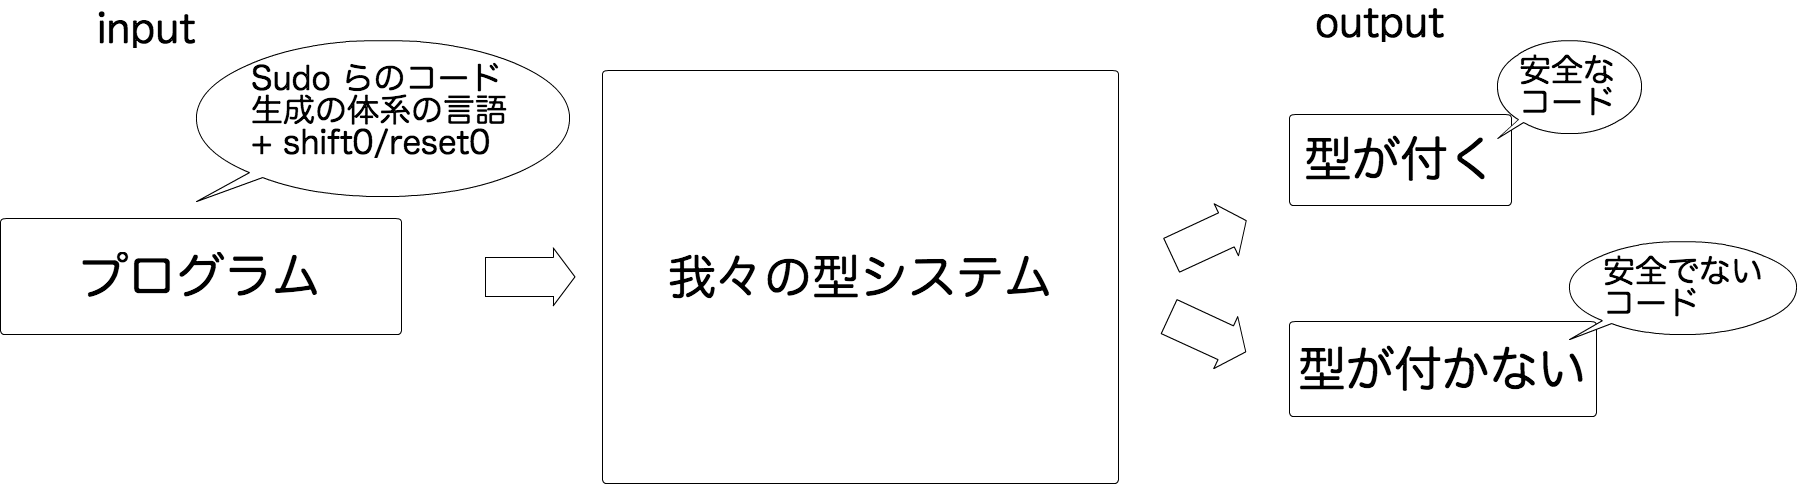
\includegraphics[clip,height=3.2cm]{./img/code_s0r0.png}
    \end{column}
  \end{columns}
\end{frame}



\subsection{コード生成器と生成されるコード}

\begin{frame}
  \center
  \huge{まず表現力について}
\end{frame}

\begin{frame}
  \frametitle{コード生成器と生成されるコード}

  \begin{onlyenv}<1>
    \begin{columns}
      \begin{column}{0.5\textwidth}%% [横幅] 0.2\textwidth = ページ幅の 20 %
        コード生成器
        \begin{align*}
          & \red{...}~ \cfordo{x = e1}{e2} \\
          & ~~\red{...}~ \cfordo{y = e3}{e4} \\
          & ~~~~\red{...}~ \magenta{\cLet~u=t~\cIn} \\
          & ~~~~~~\red{...}~ \caryset{\code{a}}{(x,y)} u
        \end{align*}
      \end{column}
      $\too$
      \begin{column}{0.5\textwidth}%% [横幅] 0.2\textwidth = ページ幅の 20 %
        生成されるコード
        \begin{align*}
          & \langle \magenta{\Let ~u' ~= ~t' ~\In} \\
          & ~~\fordo{x' = e1'}{e2'} \\
          & ~~~~\fordo{y' = e3'}{e4'} \\
          & ~~~~~~\aryset{a}{x',y'}{u'} \rangle
        \end{align*}
      \end{column}
    \end{columns}
  \end{onlyenv}
\end{frame}


% 以降はコード生成器のみの話にしぼって話します

\subsection{多段階let 挿入}

\begin{frame}
  \frametitle{shift0/reset0 によるlet挿入}

    \begin{align*}
\uncover<3->{
      \Resetz ~(E[\Shiftz~ k \to e]) &\to e \ksubst{k}{E}
}
    \end{align*}

\noindent
    \begin{align*}
    \text{コード生成器:}~~
      & \uncover<4->{\blue{\Resetz}} ~~\cfordo{x = e1}{e2} \\
      & ~~\uncover<2-3>{\blue{\Resetz}} ~~\cfordo{y = e3}{e4} \\
      & ~~~~\uncover<2->{\blue{\Shiftz}~\blue{k}~\to}~ 
            \magenta{\cLet~u=t~\cIn} \\
      & ~~~~~~\uncover<2->{(\blue{\Throw~k}}~(\caryset{a}{(x,y)}{u})
              \uncover<2->{)} \\
      &   \uncover<3,5->{\blue{k}} 
\only<3>{\Leftarrow ~~\cfordo{y = e3}{e4}~[\ ]} 
\only<5->{\Leftarrow ~~\cfordo{x = e1}{e2} ~~\cfordo{y = e3}{e4} ~~[\ ]} \\
    \text{生成コード:}~~
      & \uncover<3,5->{\langle~}
\only<3>{\fordo{x' = e1'}{e2'}} \only<5->{\magenta{\Let ~u' ~= ~t' ~\In}} \\
      & ~~ 
\only<3>{\magenta{\Let ~u' ~= ~t' ~\In}} \only<5->{\fordo{x' = e1'}{e2'}} \\
      & ~~~~\uncover<3,5->{\fordo{y' = e3'}{e4'}} \\
      & ~~~~~~\uncover<3,5->{\aryset{a}{x',y'}{u'} ~\rangle}
    \end{align*}
\end{frame}


\begin{frame}
  \frametitle{shift0/reset0 による\alert{多段階}let挿入}

    \begin{align*}
      \Resetz ~(E[\Shiftz~ k \to e]) &\to e \ksubst{k}{E}
    \end{align*}

\noindent
    \begin{align*}
    \text{コード生成器:}~~
      & \red{\Resetz} ~~\cfordo{x = e1}{e2} \\
      & ~~\blue{\Resetz} ~~\cfordo{y = e3}{e4} \\
      & ~~~~\blue{\Shiftz}~\blue{k_2}~\to~ 
            \red{\Shiftz}~\red{k_1}~\to~ 
            \magenta{\cLet~u=t~\cIn} \\
      & ~~~~~~\red{\Throw~k_1}~
              (\blue{\Throw~k_2}~(\caryset{a}{(x,y)}{u})) \\
%        & \red{k_1} \Leftarrow ~~\cfordo{x = e1}{e2}~[\ ] \\
%        & \blue{k_2} \Leftarrow ~~\cfordo{y = e3}{e3}~[\ ] \\
    \text{生成コード:}~~
      & \langle~\magenta{\Let ~u' ~= ~t' ~\In} \\
      & ~~\fordo{x' = e1'}{e2'} \\
      & ~~~~\fordo{y' = e3'}{e4'} \\
      & ~~~~~~\aryset{a}{x',y'}{u'} ~\rangle
    \end{align*}

\end{frame}

\begin{frame}
  \center
  \huge{次に安全性}
\end{frame}

\begin{frame}
  \center
  \huge{コード生成前の段階で,安全なコードかどうかを判断する}
\end{frame}

% \begin{frame}
%   \center
%   \huge{安全なコードにのみ型をつけるにはどうすればよいか}
% \end{frame}

\subsection{型システム}

\begin{frame}
  \frametitle{環境識別子(EC)を利用したスコープ表現 [Sudo+2014]}
%  \begin{center}
%    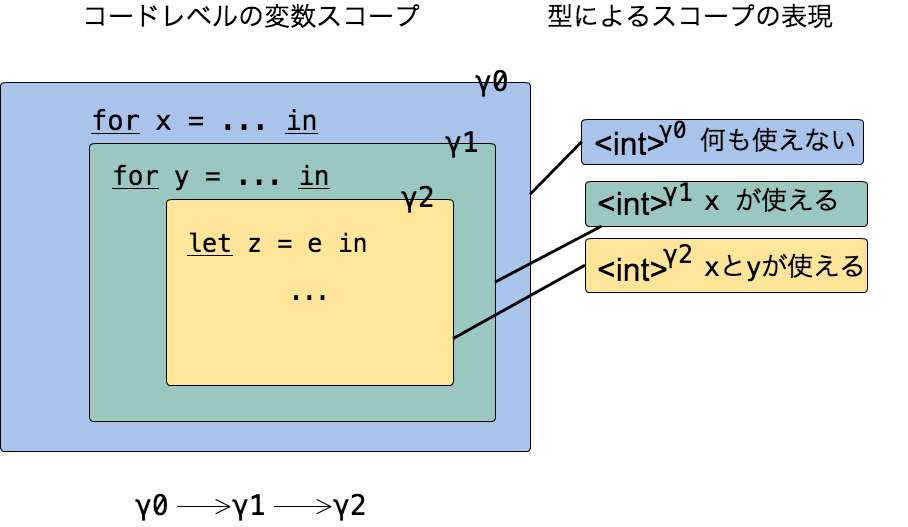
\includegraphics[clip,height=5.7cm]{./img/ec_for.png}
%  \end{center}
%  \begin{flushright}
%    $\gamma_i ... \text{Refined Environment Classifier}$
%  \end{flushright}

\newcommand\ml{\multicolumn}


{\Large
\begin{tabular}{l|l|l|l|l|l|}
\cline{2-6} 
\alert{$\mathbf \gamma0$} & \ml{5}{|l|}{\cfordo{x = e1}{e2}~~~~~~~~~~~~~~~} \\ \cline{3-5}
          & \alert{$\mathbf \gamma1$} & \ml{3}{|l|}{\cfordo{y = e1}{e2}} & \\ \cline{4-4}
          &           & \alert{$\mathbf \gamma2$} & \ml{1}{|l|}{\caryset{a}{(x,y)}~t} & ~~ & \\ \cline{4-4}
          &           & \ml{3}{|l|}{\ }    &               \\ \cline{3-5}
          & \ml{5}{|l|}{~~~~~~~~~~~~~~~~~~ } \\ \cline{2-6}
\end{tabular}
}

\begin{center}
\begin{tabular}{c|c}
スコープ & 使えるコード変数 \\ \hline
$\gamma0$ & なし \\ \hline
$\gamma1$ & x \\ \hline
$\gamma2$ & x,y
\end{tabular}\qquad
\end{center}

\end{frame}

\begin{frame}
  \frametitle{環境識別子(EC)を利用したスコープ表現 [Sudo+2014]}

型システムでコード変数のスコープを表現:
\begin{align*}
\gamma2 \ord \gamma1,~
x : \codeTs{\textbf{int}}{\gamma1},~
y : \codeTs{\textbf{int}}{\gamma2}
& ~\vdash~ x : \codeTs{\textbf{float}}{\gamma2}  & \alert{\text{OK}}
\\
\gamma2 \ord \gamma1,~
x : \codeTs{\textbf{int}}{\gamma1},~
y : \codeTs{\textbf{int}}{\gamma2}
& ~\vdash~ y : \codeTs{\textbf{float}}{\gamma1}  & \alert{\text{NG}}
\\
\gamma2 \ord \gamma1,~
x : \codeTs{\textbf{int}}{\gamma1},~
y : \codeTs{\textbf{int}}{\gamma2}
& ~\vdash~ x\cPlus y : \codeTs{\textbf{int}}{\gamma2}  & \alert{\text{OK}}
\end{align*}

コードレベルのラムダ抽象の型付け規則で,固有変数条件を利用:

  \[
    \infer[(\gamma_2~\text{is eigen var})]
    {\Gamma \vdash \cfun{x}{e} : \codeTs{t_1\to t_2}{\gamma_1} }
    {\Gamma,~\gamma_2 \ord \gamma_1,~x:\codeTs{t_1}{\gamma_2} \vdash 
      e : \codeTs{t_2}{\gamma_2}}
  \]

\end{frame}

\begin{frame}
  \frametitle{環境識別子(EC)を利用したスコープ表現}

先行研究:
\begin{itemize}
\item 局所的なスコープをもつ破壊的変数をもつコード生成の体系に対する(型安全な)型システムの構築
 [Sudo,Kiselyov,Kameyama 2014]
\item グローバルなスコープをもつ破壊的変数への拡張 
 [Kiselyov,Kameyama,Sudo 2016]
\item コントロールオペレータには非対応
\end{itemize}

\medskip
問題点:
shift0/reset0 などのコントロールオペレータは,スコープの包含関係を逆転させてしまう.
\end{frame}

\begin{frame}
ここに,forループとshift0/reset0 の例を再掲する.

もとのスライドの 24ページの絵をかく.
\end{frame}

\begin{frame}
\frametitle{本研究での解決策}

3つのアイディア:
\begin{itemize}
\item 包含関係にないEC 
\item ジョイン演算子
\item EC に関する多相性
\end{itemize}

\end{frame}


\begin{frame}
  \frametitle{ECのジョイン}
  \flushleft
  
\includegraphics[clip,height=3cm]{./img/ecgraph.png}
  \begin{itemize}
  \item<2-> $\gamma_1$ のコードレベル変数は $\gamma_2$ では使えない
  \item<3-> $\gamma_2$ のコードレベル変数は $\gamma_1$ では使えない
  \item<4-> $\gamma_1, \gamma_2$ のコードレベル変数は $\gamma_3$ で使える
  \item<5->[$\Rightarrow$] Sudoらの体系に $\cup$ を追加
  \end{itemize}
\end{frame}

\begin{frame}[fragile]
  \frametitle{コード生成+shift0/reset0 の型システム (の一部)}
  コードレベルのラムダ抽象:
  \[
    \infer[(\gamma_1~\text{is eigen var})]
    {\Gamma \vdash \cfun{x}{e} : \codeT{t_1\to t_2}{\gamma} ~;~ \sigma}
    {\Gamma,~\gamma_1 \ord \gamma,~x:\codeT{t_1}{\gamma_1} \vdash e
      : \codeT{t_2}{\gamma_1}; \sigma}
  \]

  reset0:
  \[
    \infer{\Gamma \vdash \resetz{e} : \codeT{t}{\gamma} ~;~ \sigma}
    {\Gamma \vdash e : \codeT{t}{\gamma} ~;~ \codeT{t}{\gamma}, \sigma}
  \]

  shift0:
  \[
    \infer{\Gamma \vdash \shiftz{k}{e} : \codeT{t_1}{\gamma_1} ~;~ \codeT{t_0}{\gamma_0},\sigma}
    {\Gamma,~k:\contT{\codeT{t_1}{\gamma_1}}{\codeT{t_0}{\gamma_0}}{\sigma}
      \vdash e : \codeT{t_0}{\gamma_0} ; \sigma
      & \Gamma \models \gamma_1 \ord \gamma_0
    }
  \]

  throw:
  \[
  \infer
  {\Gamma,~k:\contT{\codeT{t_1}{\gamma_1}}{\codeT{t_0}{\gamma_0}}{\sigma}
    \vdash \throw{k}{v} : \codeT{t_0}{\gamma_2} ; \sigma}
  {\Gamma
    \vdash v : \codeT{t_1}{\gamma_1 \cup \gamma_2} ; \sigma
    & \Gamma \models \gamma_2 \ord \gamma_0
  }
\]

\end{frame}


%%% Local Variables:
%%% mode: japanese-latex
%%% TeX-master: "slide"
%%% End:
